\section{Konstruktion und 3D-Druck des Entwurfs}
The final design differs significantly from the prototypes. It has seen many iterative improvements and thus deserves its' own chapter to cover all the changes to each component of the design. The final design consists of the following bodies:
\begin{enumerate}
	\item{\textbf{Stand}} Is the stand upon which the device resides. Needed for introduction an another axis of rotation and decoupling dispense and disposal mechanisms
	\item{\textbf{UpperBody}} Consists of a walls and a floor of a dispense mechanism with a cutout for dispene and disposal paths as well as connection mechanisms.
	\item{\textbf{UpperMill}} Is a mechanisms that divides the whole dispense system into 21 functional + 1 service chamber (22 in total). Inner side contains a gear and teeth for connecting upper mill with the lower mill (synchronicity between them is still retained)
	\item{\textbf{LowerMill}} Is a mechanisms that divides the whole disposal system into 22 chambers. Unlike dispense system, they are all the same, since chambers need to be of the same size as dispense system, but there is no need for the service chamber. it also contains grooves to reduce the surface contact with lower body and thus friction
	\item{\textbf{LowerBody}} is a very complex detail. Firstly, it contains cutouts for the stepper motor, driver and the deck that holds further electronics. Secondly, it has "ears" that define the axis of rotation for the dispense pathway. Thirdly, it contains grooves for the lower mill to travel on rotationally, to optimize power spent on overcoming friction.
	\item{\textbf{LowerDeck}} Is a cover for all the electronics inside. It contains grooves on the sides for it to slide into electronics chamber.
	\item{\textbf{Electronics}} is the housing for microcontrooler, battery and charger. it also contains cutout for the deck to slide into so that electronics is covered from the outside.
	\item{\textbf{Holder}} is a mechanism of additional mechanical fixation of the electronics. Although the Electronics compartment was designed so, that all the components are fixed in place, it might come to the situations where excess movement (e.g. during transportation) might cause electronics to fall out. this mechanism prevents it.
	\item{\textbf{UpperDeck}} Is an upper cover of the device.
\end{enumerate}

Moving forward, we will go step-by-step into the design of each of those components and also will cover the nuances of 3D-printing them all. For now, however, we will compare the final design with the goals set and why this design was chosen in the end. The goals can be divided into 2 types: Initial requirements and the problems arisen during previous designs. Initial requirements are:
\begin{enumerate}
	\item{\textbf{Das Gerät enthält 21 Kammern, 3 für jeden Tag der Woche}} This requirement is satisfied. The final design has 22 chambers, 21 of which can contain pills.
	\item{\textbf{Das Gerät enthält ein Pillenrücknahmesystem}} This requirement is also satisfied. 
	\item{\textbf{Das Gerät verfügt über eine begleitende App zur Fernsteuerung.}} This is not implemented yet. Alternatively, this requirement tells us, that an user interface on the body of device itself is not required. The electronics of this device are chosen so that this requirement can be implemented later on.
\end{enumerate}
The problems that arisen during the design are solved:
\begin{enumerate}
	\item{From first prototype:}
	\begin{enumerate}
		\item{\textbf{Zu viele bewegliche Teile}} Final design only has 2 mills that are moving simultaneosly on the same axis and nothing else. This is significant improvement over the first design
		\item{\textbf{Erfordert eine große Spenderschale}} the disposal system of the final design is located directly underneath the dispensing system and they have the same spatial dimensions.
		\item{\textbf{Enthält mehrere kleine Objekte}} The only small object is the holder, all the other ones are big and static, which reduces the amount of potential failure points.
	\end{enumerate}
	\item{From first prototype:}
	\begin{enumerate}
		\item{\textbf{Chambers of the upper mechanism are smaller}} Since the dispense and disposal mechanisms are of the same size, this is not the problem
		\item{\textbf{Synchronous movement of both chambers}} While both mechanisms still move synchronically, the pathways of dispense and disposal were decoupled, therefore their synchronous movement is not a problem anymore.
		\item{\textbf{Reliance on a ramp for pills to fall down.}} The final design doesn't have a ramp. the pills would fall directly down in the disposal pathway. In dispense pathway, the device would be tilted 45 degrees which makes certain that the pills would fall down.
	\end{enumerate}
	\item{From third prototype:}
	\begin{enumerate}
		\item{\textbf{Too tall}} The device will never be completely vertical. Although the device is now at an elevation it is still shorter as when having to have one wheel aways be vertical.
		\item{\textbf{Requires more Rotational momentum}} since both mills are now horizontal, there is no extra power spent to battle gravity. the mills will only normally rotate in horizontal position.
	\end{enumerate}
\end{enumerate}
\newpage
\subsection{Components of the final design}
\subsubsection{UpperBody}
\begin{figure}[h]
	\centering
	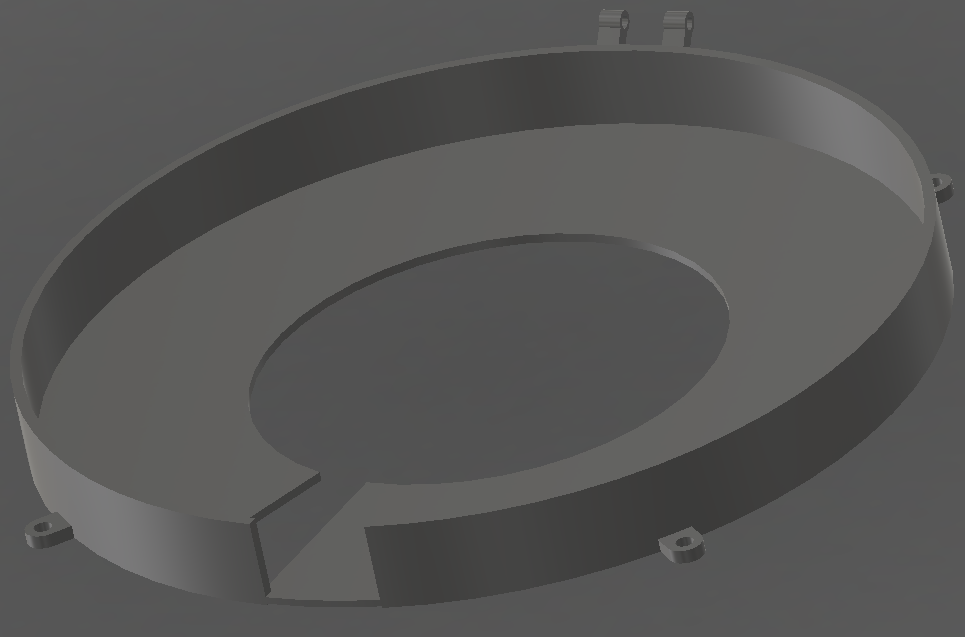
\includegraphics[width=0.7\linewidth]{Figures/Screenshot_6}
	\caption[Upper Body]{Upper Body}
	\label{fig:screenshot6}
\end{figure}
Upper body is a simple design consisting of a cylindrical shape with multiple cutouts. First one is on the floor, through this hole the pills that have not been taken would fall. The other cutout is in the wall, through this cutout the pills that will have to be taken would fall. In the middle there is a circular hole for housing the mill. 

The measurements are:
\begin{itemize}
	\item outer radius = 100mm
	\item inner radius = 52 mm
	\item height = 20 mm
	\item thickness of floor = 2 mm
	\item thickness of wall = 2.5 mm 
\end{itemize}
\newpage
\subsubsection{UpperMill}
\begin{figure}[h]
	\centering
	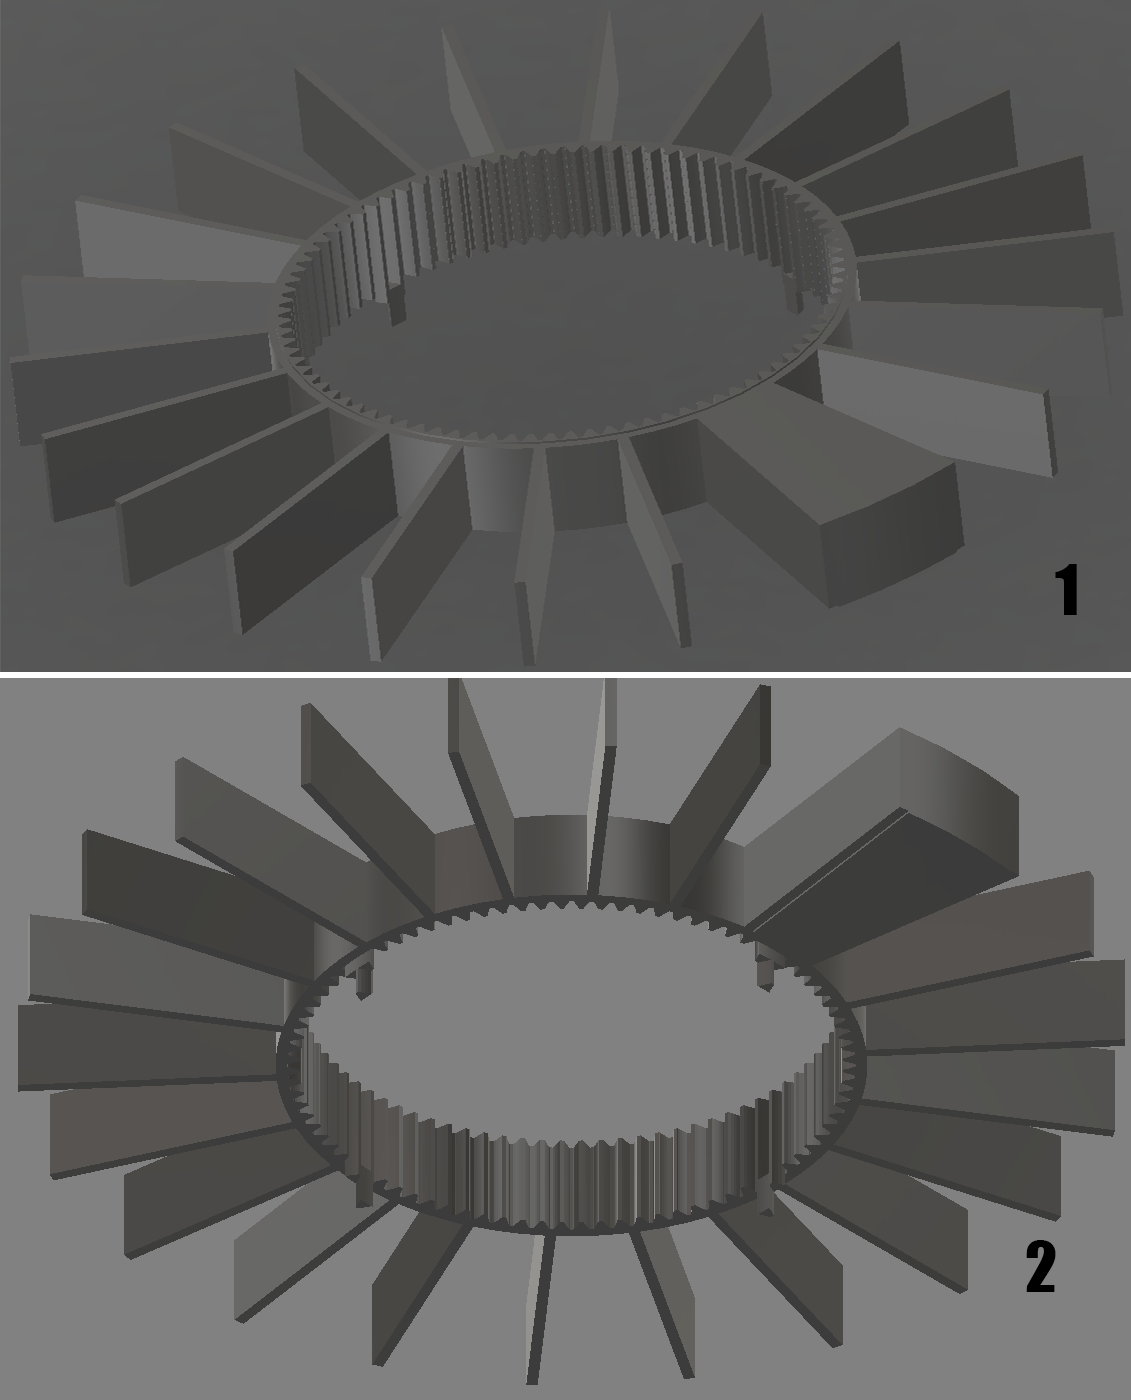
\includegraphics[width=0.6\linewidth]{Figures/Uppermill}
	\caption[Upper Mill]{Upper Mill. 1 View from above. 2 view from below}
	\label{fig:uppermill}
\end{figure}
Upper mill consists of 21 functional chambers and one service chamber. the service chamber is needed to cover the hole in the upper body, so that at any time, 21 chambers are available. Inner rim is designed as a  zahnrad. It has 88 teeth, it will be important later for the stepper motor movement calculation. The gear was designed using a free tool called DXF and SVG GEAR DXF GENERATOR \cite{evolvent_spur_gear_generator}.
These parameters were chosen to match the size of the cog and amount of teeth needed: 
\begin{itemize}
	\item Gear 1 Tooth Count: $-88$ (internal gear)
	\item Gear 2 Tooth Count: $22$
	\item Module: $1.11$ (mm)
	\item Pressure Angle: $20^\circ$
	\item Clearance: $0.15$ mm
	\item Gear 1 Center Hole Diameter: $0$ mm (no hole)
	\item Gear 2 Center Hole Diameter: $0$ mm (no hole)
\end{itemize}

The lower side contains 4 teetch to connect the upper mill to the lower mill. This implementation makes sure that the two mills will move at the same time, removing need for a separate stepper motor for each of them or a connection directly to the upper mill.

There are certain design decisions that have been taken to reduce friction. Firstly, on the upper side the ring is offset by 0.4 mm so that the upper deck will not touch the whole mechanism, but only this ring. At the bottom side, the teeth are complex shaped. the upper part of the tooth has a length of 2.4 mm, which is 0.4 mm taller than the thickness of the floor of the upper body. The idea behind it is that the wings of the mill will not touch the floor directly, leaving 0.2 mm opening between the floor and the upper mill.
 
The measurements of the upper mill are:
\begin{itemize}
	\item chamber height = 17 mm
	\item[] chamber length = 45.05 mm
	\item inner ring diameter = 100 mm
	\item outer ring diameter = 193 mm
	\item gear tooth depth 2.7 mm
	\item connecting tooth length = 2.4 mm + 5 mm
\end{itemize}
\newpage
\subsubsection{LowerMill}
\begin{figure}[h]
	\centering
	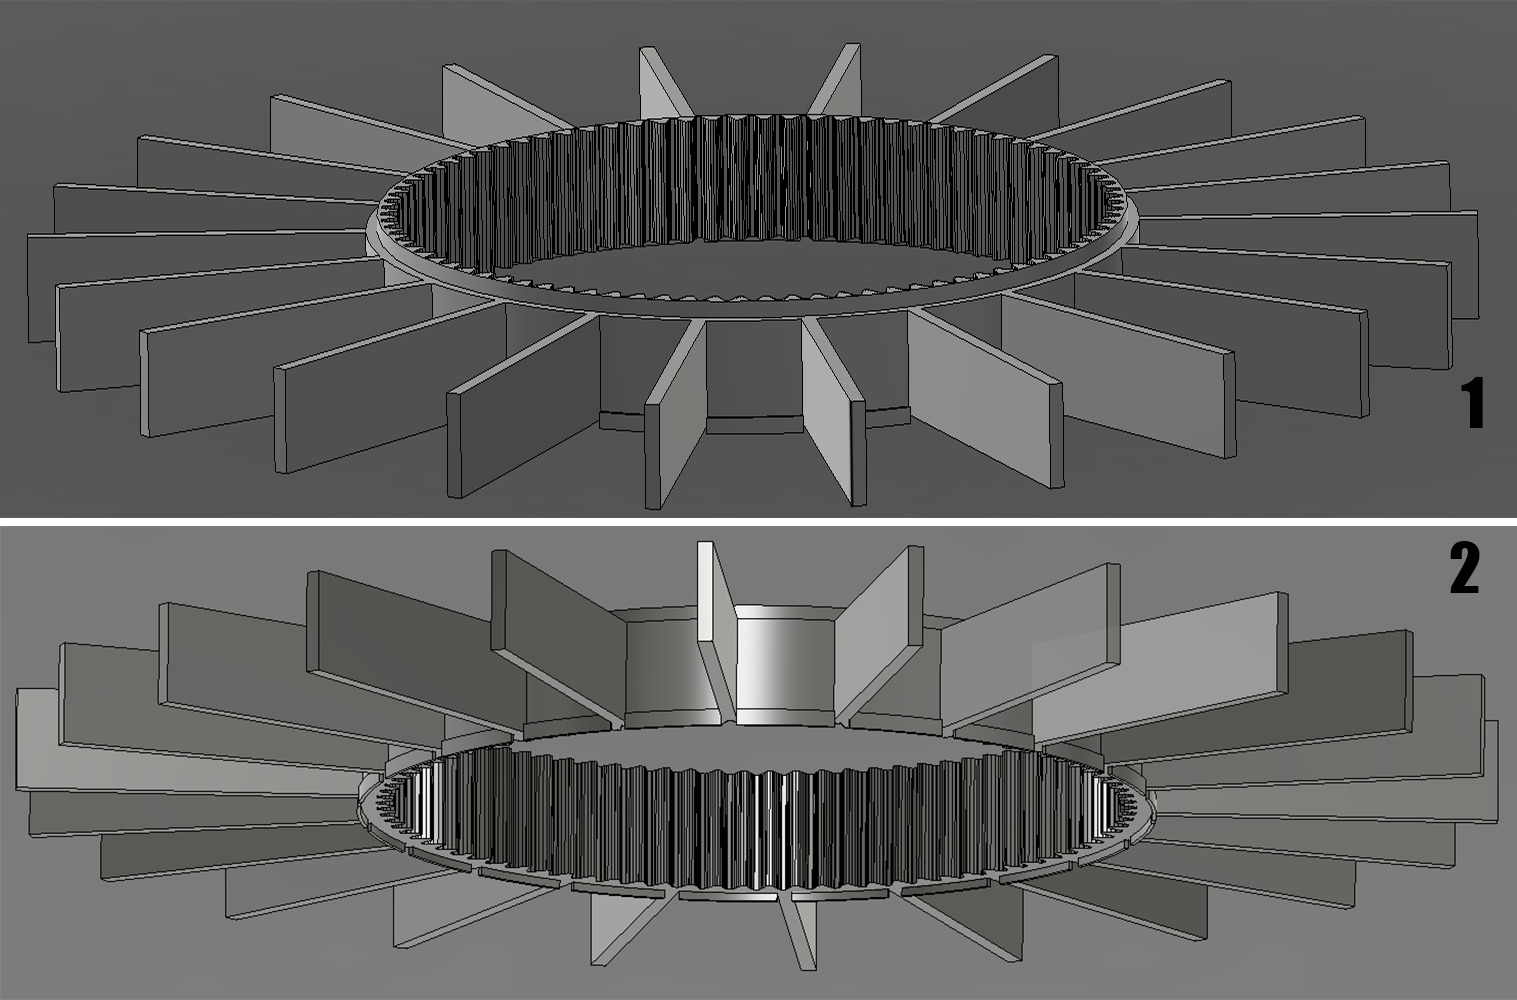
\includegraphics[width=0.7\linewidth]{Figures/Lowermill}
	\caption[Lower Mill]{Lower mill. 1 view from above. 2 view from below}
	\label{fig:lowermill}
\end{figure}
Lower mill consists of 22 chambers which are the same. This is done to make sure that the sizes of upper and lower mill chambers are the same. Just as with the upper mill, inner ring is also a zahnrad, designed the same way and with the same parameters as upper mill. Unlike the upper mill, lower mill doesn't have teeth to connect. The teeth of upper mill are inserted into teeth of zahnrad of the lower mill.

The upper part also contains a ring that is 2 mm above the rest of the construction. This ring exists to eliminate the friction between the ceiling (which is a floor of the upper mill) and the chambers. 

The lower part is also made in such a way as to reduce friction. it contains rims that would travel rotationally along the ring located on the lower body. they are rather tall, measured at 1 mm to make sure that they don't accidentally fall out during movement.

The measurements of lower mill are:
\begin{itemize}
	\item chamber height = 13.6 mm
	\item[] chamber length = 45.05 mm
	\item inner ring diameter = 100 mm
	\item outer ring diameter = 193 mm
	\item gear tooth depth 2.7 mm
\end{itemize}
\subsubsection{LowerBody}
\subsubsection{Electronics}
\subsubsection{LowerDeck}
\subsubsection{Stand}
\subsection{3D printing specifics}
